\documentclass{beamer}

\mode<presentation>
{
  \usetheme{metropolis}
  \usecolortheme{default}
  \usefonttheme{default}
  \setbeamertemplate{navigation symbols}{}
  \setbeamertemplate{caption}[numbered]
}

\usepackage[czech]{babel}
\usepackage[utf8x]{inputenc}
\usepackage{tikz}

\usetikzlibrary{fit}
\usetikzlibrary{positioning}
\usetikzlibrary{arrows.meta}
\usetikzlibrary{backgrounds}

\title[RoFi]{RoFi}
\author{Jan Mrázek, Viktória Vozárová}
\institute{Paradise}
\date{21. 5. 2018}

\begin{document}

\begin{frame}
  \titlepage
\end{frame}

\begin{frame}{Co je naším cílem?}

    Vyvinout rekonfigurovatelnou distribuovanou robotickou platformu.

    \pause

    \begin{center}
    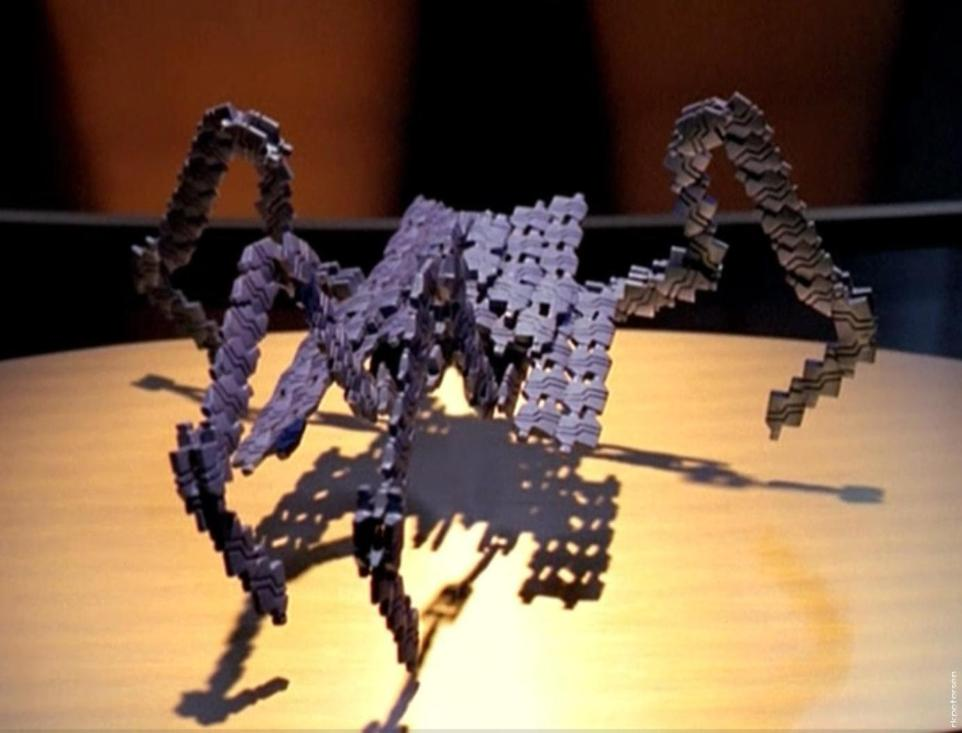
\includegraphics[width=0.6\textwidth]{img/replicator2}

    ...v podstatě Replikátory z StarGate SG-1.

    \url{https://youtu.be/gm0KUVByx40?t=49}
    \end{center}

\end{frame}

\begin{frame}{Co je to replikátor?}
    \begin{center}
        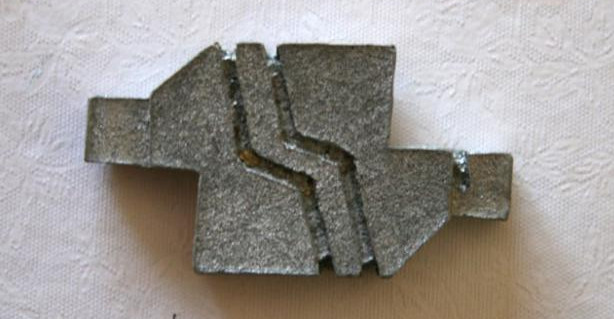
\includegraphics[width=0.6\textwidth]{img/replicator3}
    \end{center}

    \begin{columns}
        \begin{column}{0.5\textwidth}
            Co si bereme jako inspiraci:
        \end{column}
        \begin{column}{0.5\textwidth}
            \only<2->{Čemu se chceme vyvarovat:}
        \end{column}
    \end{columns}

    \begin{columns}
        \begin{column}{0.5\textwidth}
            \begin{itemize}
                \item rekonfigurovatelnost
                \item distribuovanost
                \item fault tolerantnost
                \item integraci s prostředím
            \end{itemize}
        \end{column}
        \begin{column}{0.5\textwidth}
            \only<2->{
                \begin{itemize}
                    \item přílišná autonomnost
                    \item snaha se ovládnout svět
                \end{itemize}
            }
        \end{column}
    \end{columns}
\end{frame}

\begin{frame}{RoFi aka pozemský replikátor}
    \centering
    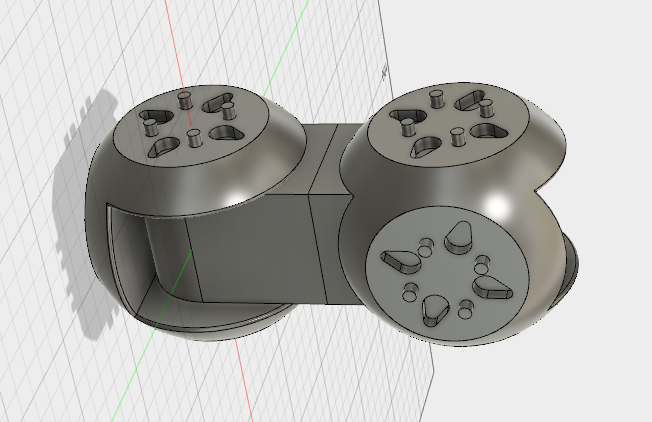
\includegraphics[width=\textwidth]{img/rofi2}
    \url{https://a360.co/2KFIRaF}
\end{frame}

\begin{frame}{Jak unikátní jsme?}
    \centering
    \only<2>{
        \begin{block}{MTRANS}
            \begin{figure}
                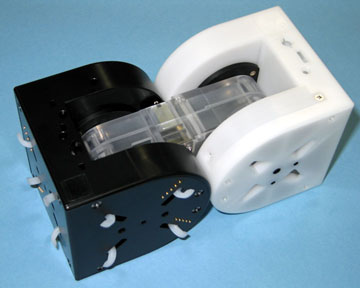
\includegraphics[width=0.7\textwidth]{img/mtran1}
            \end{figure}
        \end{block}
    }

    \only<3>{
        \begin{block}{SMORES}
            \begin{figure}
                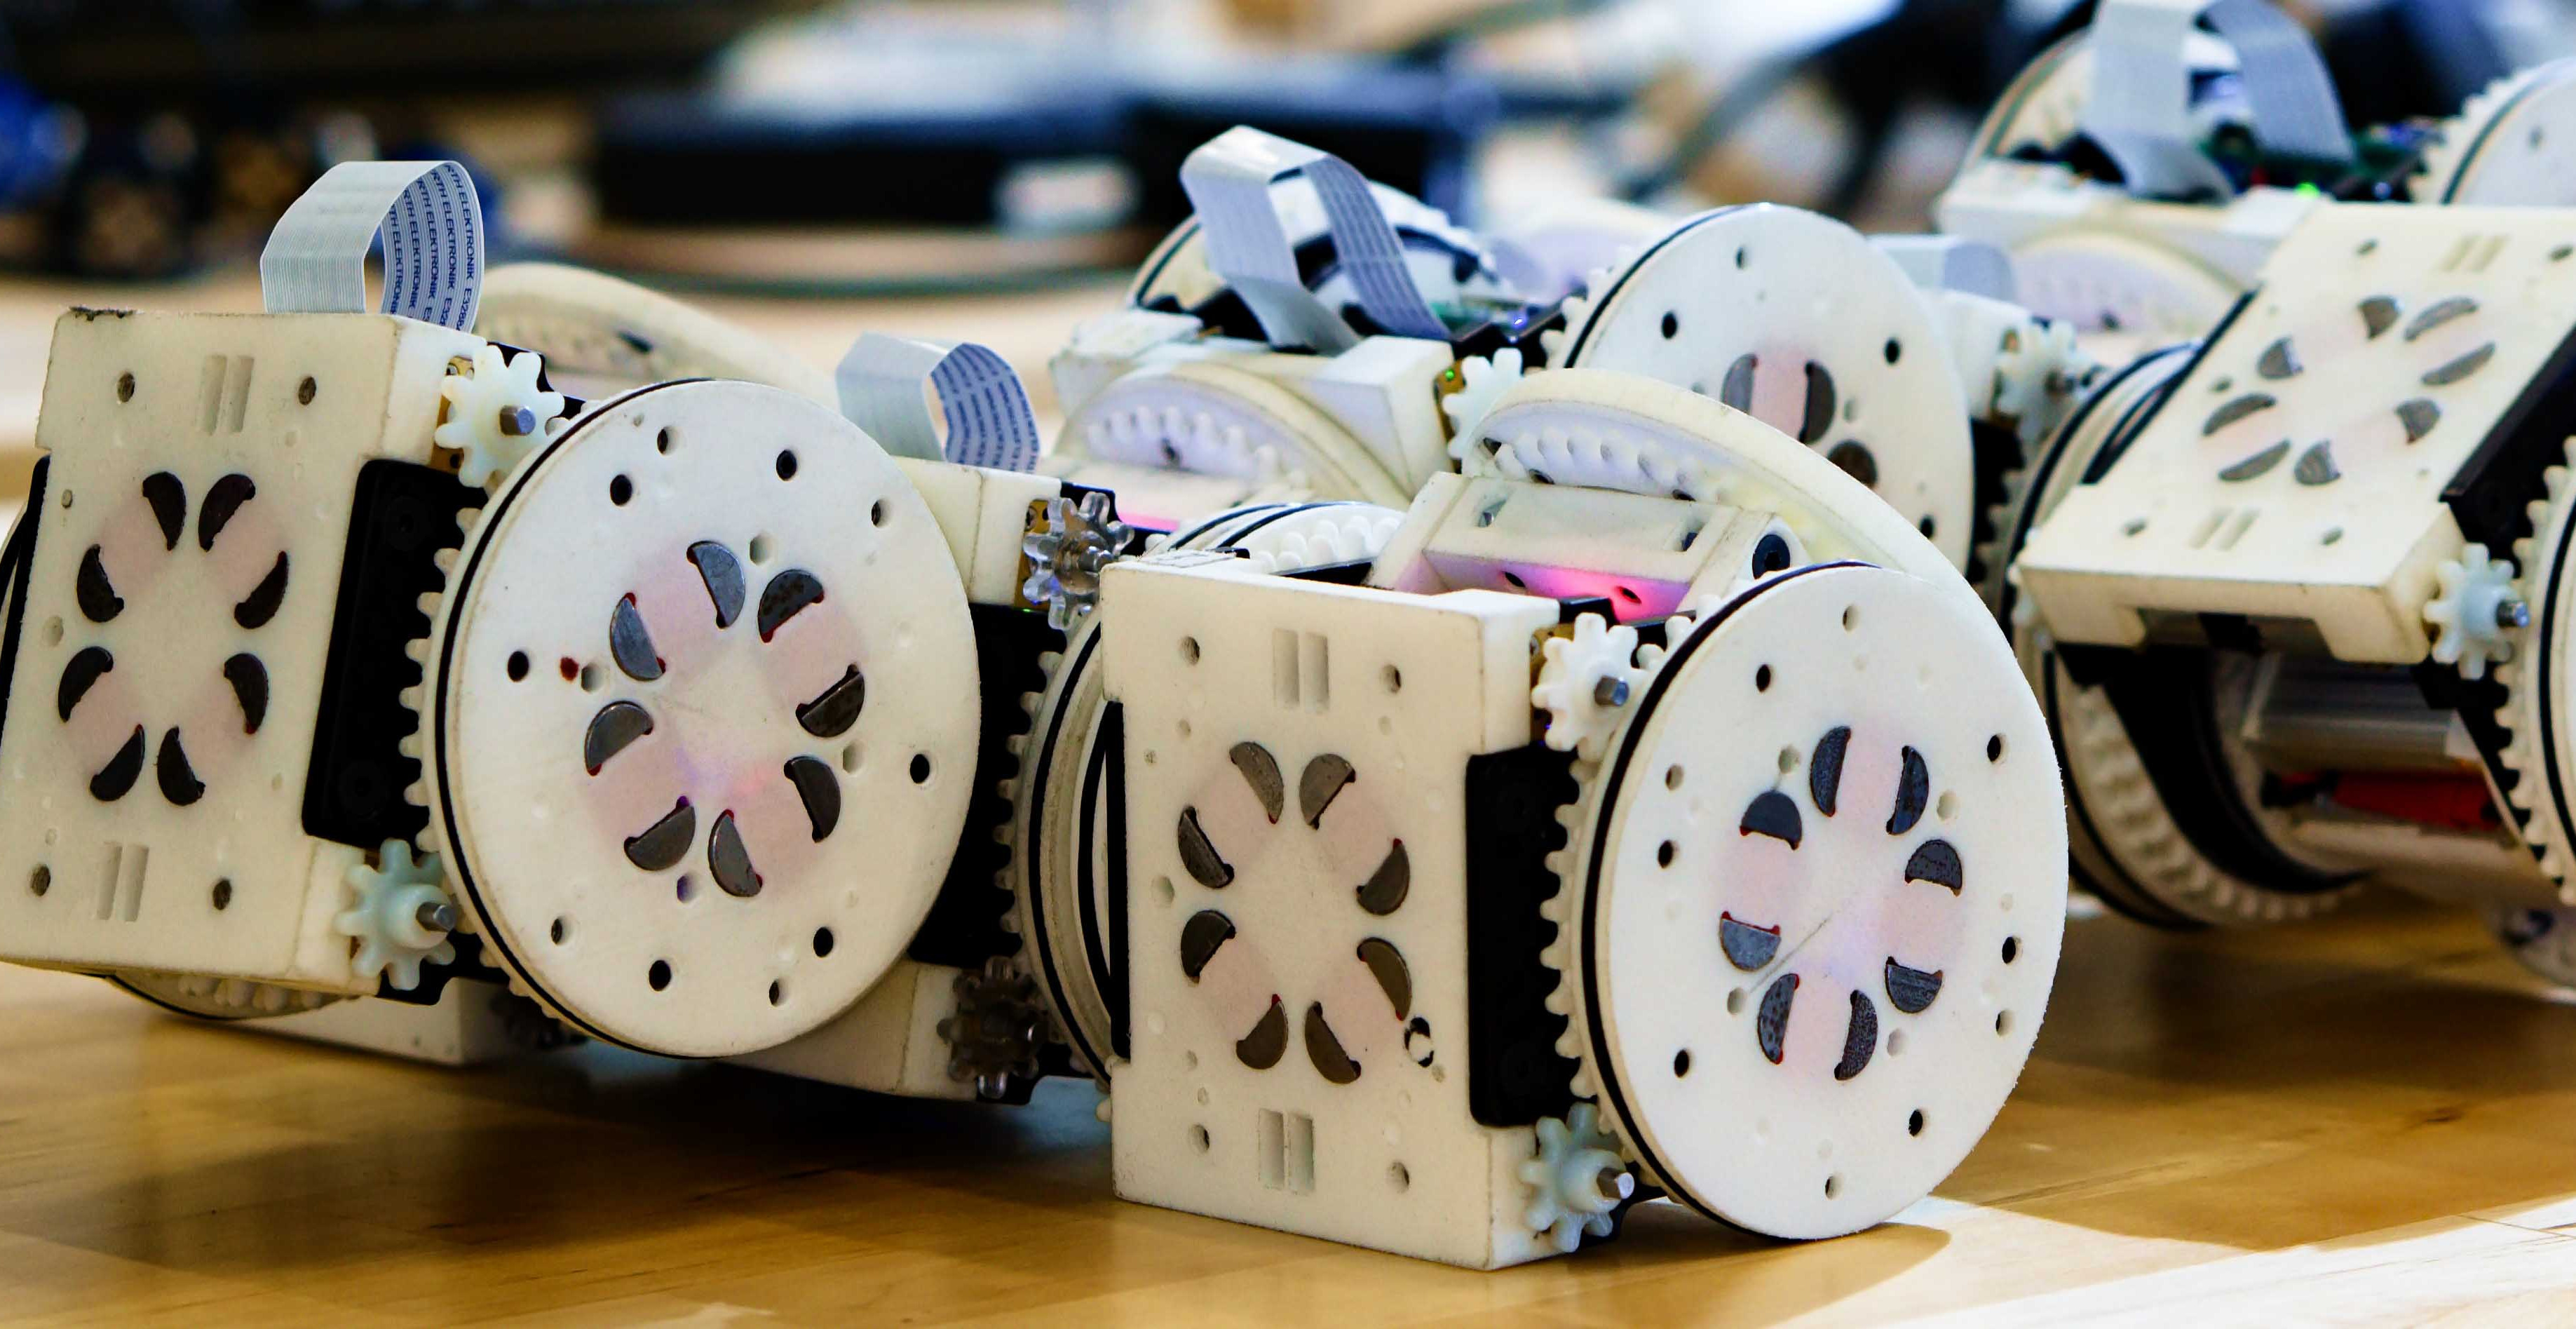
\includegraphics[width=0.8\textwidth]{img/smores1}
            \end{figure}
        \end{block}
    }

    \only<4>{
        \begin{block}{Roombots}
            \begin{figure}
                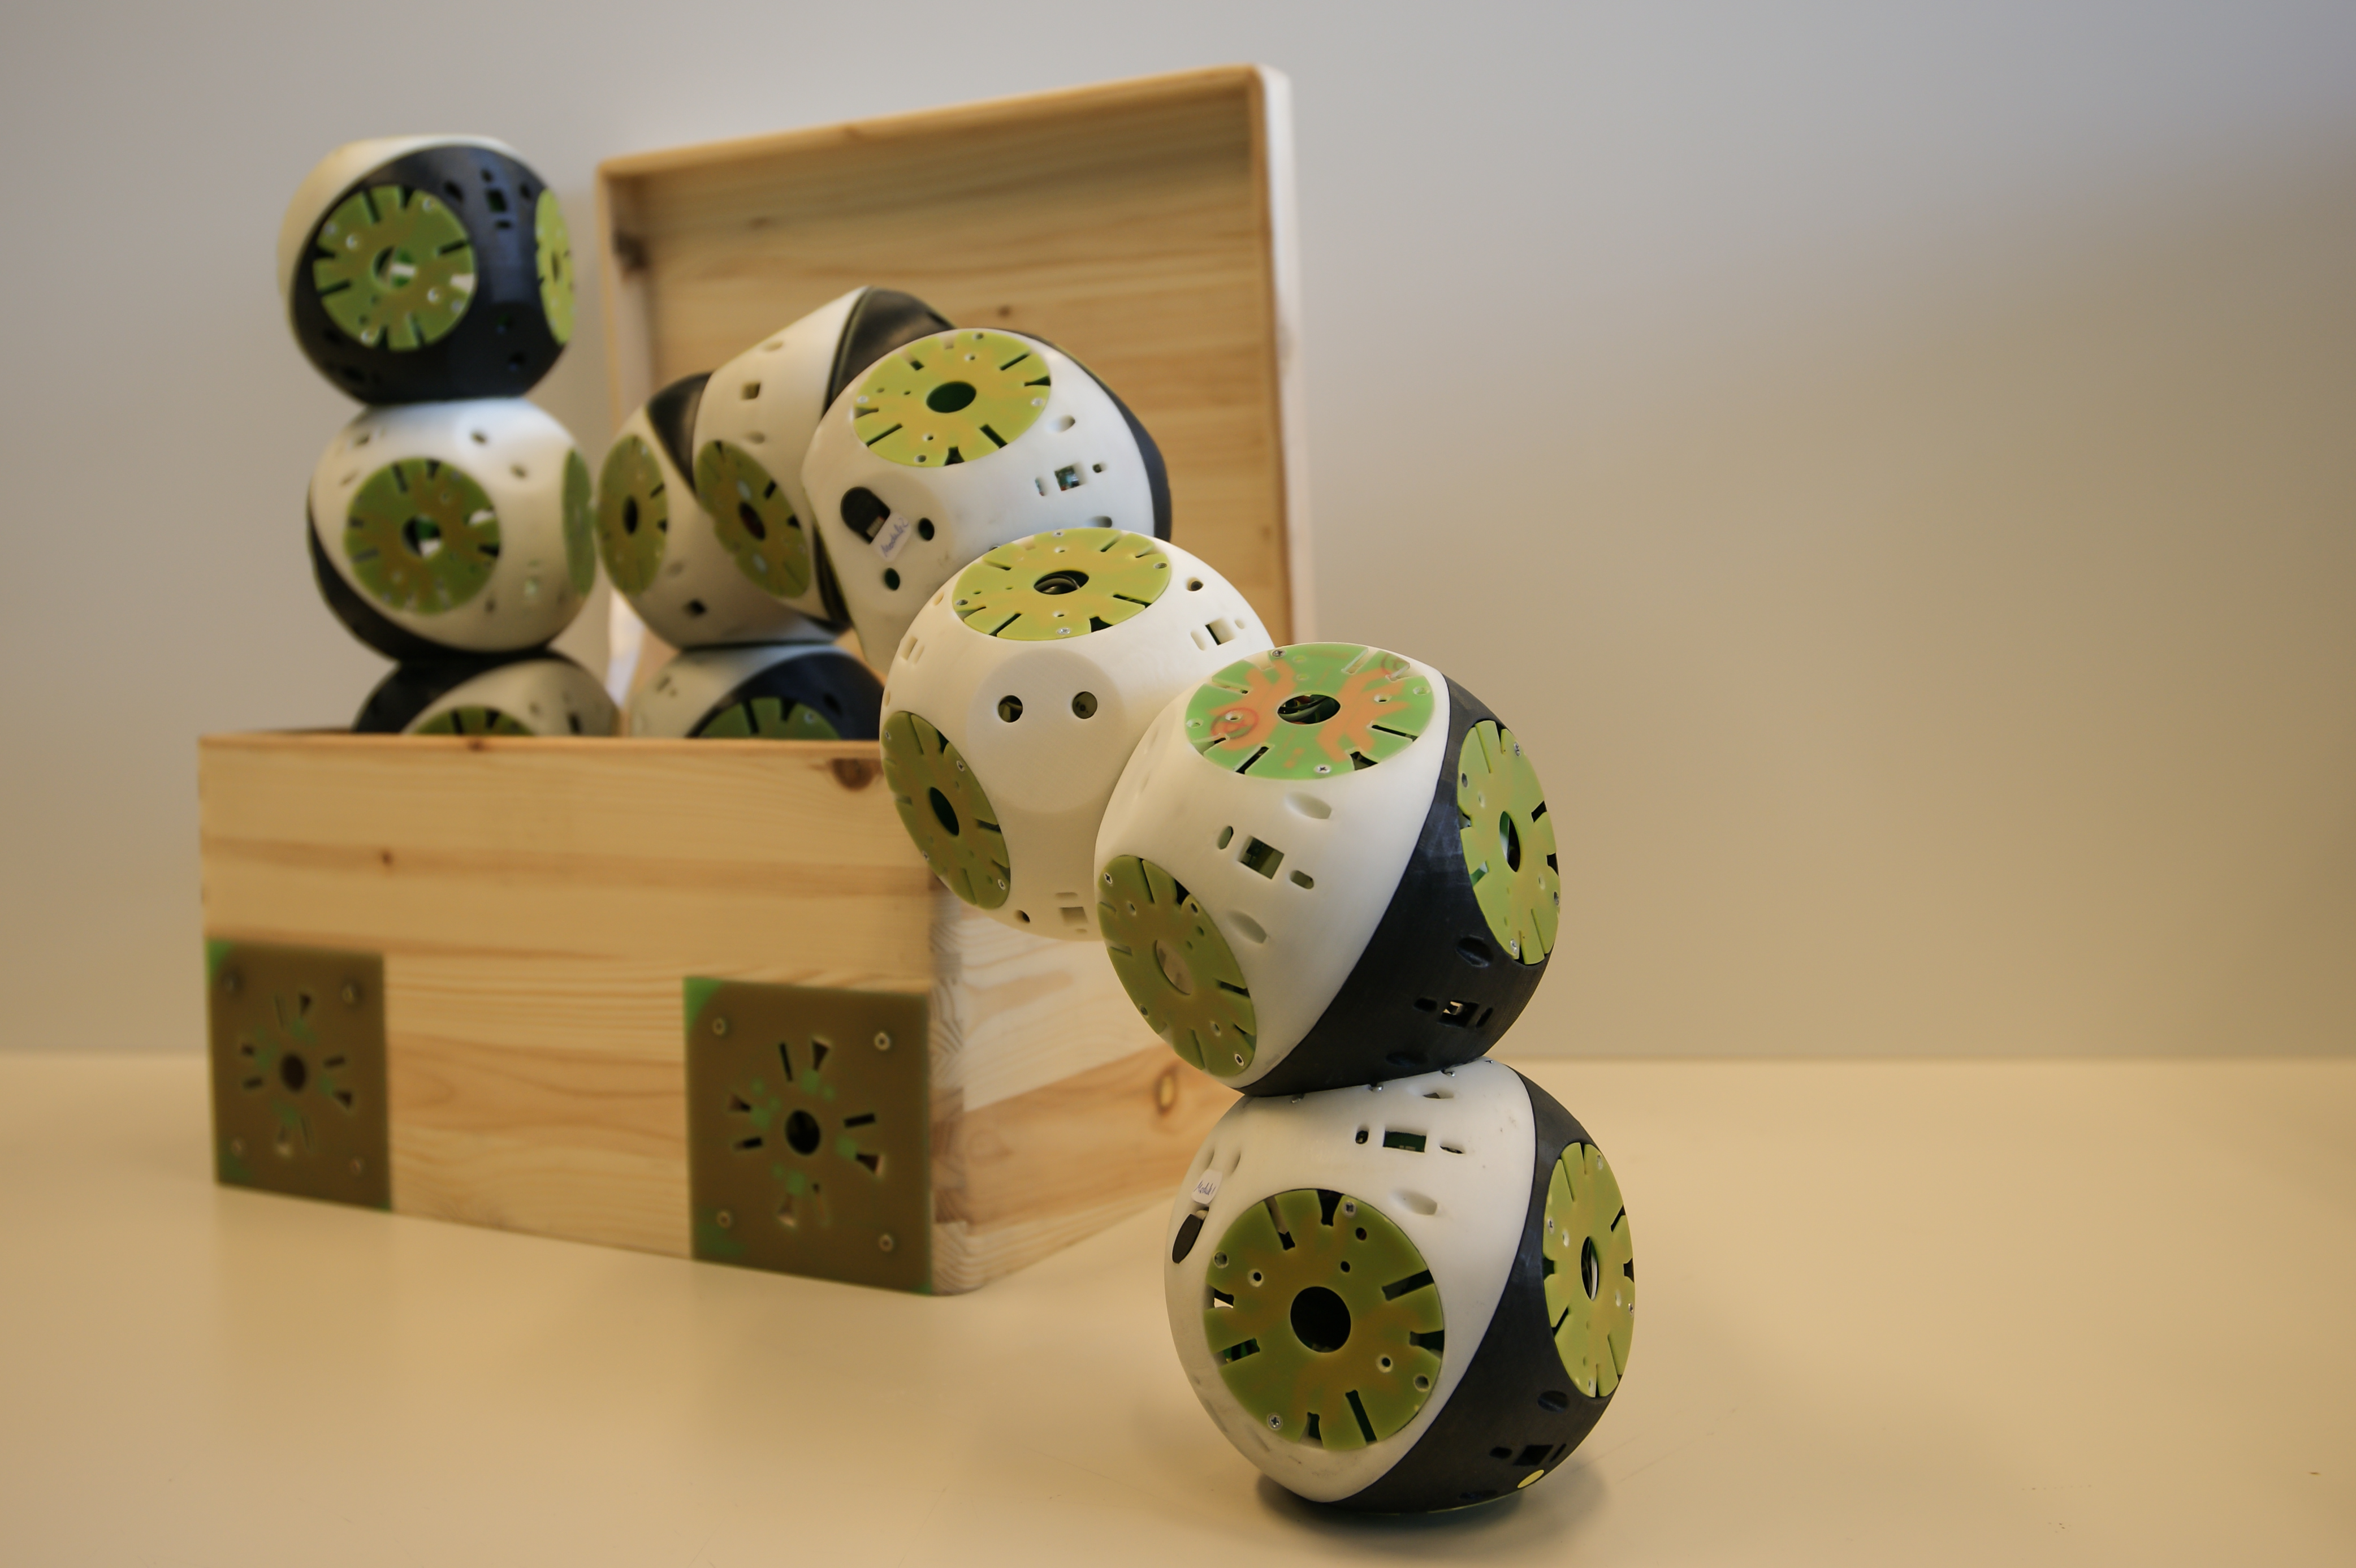
\includegraphics[width=0.8\textwidth]{img/roombot1}
            \end{figure}
        \end{block}
    }

\end{frame}

\begin{frame}{Vize projektu}
    \centering
    \resizebox {!} {7.5cm}
    {
        \begin{tikzpicture}
            \tikzstyle{hw_node}=[rectangle, draw, minimum width=2.5cm, minimum height=1cm, node distance=0.2cm, align=center, fill = white];
            \tikzstyle{os_node}=[hw_node, minimum width=1cm];

            % HW column
            \node(hw_label) [] {RoFi HW};
            \node(motors) [hw_node, below = of hw_label] {Servomotors};
            \node(mechanics) [hw_node, below = of motors] {Mechanics};
            \node(mcu) [hw_node, below = of mechanics] {Control unit};
            \node(power) [hw_node, below = of mcu] {Power mgt};
            \node(rofi_hw) [hw_node, fit=(hw_label)(power), fill=none] {};
            \scoped[on background layer]    {
                \fill[black!15] (rofi_hw.south west) rectangle (rofi_hw.north east);
            }

            % Simulator
            \node(simulator)[hw_node, below = of rofi_hw, minimum width = 2.75cm] {Simulator};

            % OS column
            \node(os_label) [right = 1.1cm of hw_label] {RoFi OS};
            \node(motion) [os_node, below left = 0.2cm and -0.7cm of os_label, minimum height = 2.8cm] {\rotatebox{90}{Motion control}};
            \node(os_dummy) [minimum width = 1cm, below = 0cm of motion] { };
            \node(communication) [os_node, below = of motion, minimum height = 2.8cm] {\rotatebox{90}{Communication}};
            \node(reconfiguration) [os_node, right = of os_dummy, minimum height = 5.8cm] {\rotatebox{90}{Reconfiguration and algorithms}};
            \node(rofi_os) [os_node, fit=(os_label)(communication)(reconfiguration), fill=none] {};
            \scoped[on background layer]    {
                \fill[black!15] (rofi_os.south west) rectangle (rofi_os.north east);
            }

            % Vertical line
            \node(vline_c) [right = 0.2cm of rofi_os] {};
            \node(vline_a) [above = 3.5cm of vline_c] {};
            \node(vline_b) [below = 3.5cm of vline_c] {};
            \draw [dashed] (vline_a) -- (vline_b);

            % Future
            \tikzstyle{future}=[rectangle, draw, rounded corners, node distance=0.5cm, fill=white];
            \node(neur) [future, right = 2cm of rofi_os] {NeuRoFi};
            \node(cv) [future, below = of neur] {RoFiCV};
            \node(passive) [future, below = of cv] {Passive components};
            \node(iorofi) [future, above = of neur] {IoRoFi};
            \node(synth) [future, above = of iorofi] {Strategy synthesis};
            \node(etc) [node distance = 0.5cm, below = of passive] {\rotatebox{90}{...}};

            \tikzstyle{arrow}=[to path={-| (\tikztotarget)}, {Latex[length=3mm]}-];
            \draw[arrow] (synth) edge (rofi_os.east);
            \draw[arrow] (neur) edge (rofi_os.east);
            \draw[arrow] (cv) edge (rofi_os.east);
            \draw[arrow] (passive) edge (rofi_os.east);
            \draw[arrow] (iorofi) edge (rofi_os.east);

            % time
            \node(time_c) [below = 0.5cm of vline_b] {};
            \node(time_begin) [left = 6.5cm of time_c] {};
            \node(time_end) [right = 5cm of time_c] {};
            \draw[arrow] (time_end) edge (time_begin);

            \node(now) [above left = 0cm and 1.4cm of time_c] {Short term plans};
            \node(vision) [above right = 0cm and 1.5cm of time_c] {Future/visions};
        \end{tikzpicture}
    }
\end{frame}

\section{Evoluce RoFi}

\begin{frame}{První koncept -- Kostičky}
    \centering
    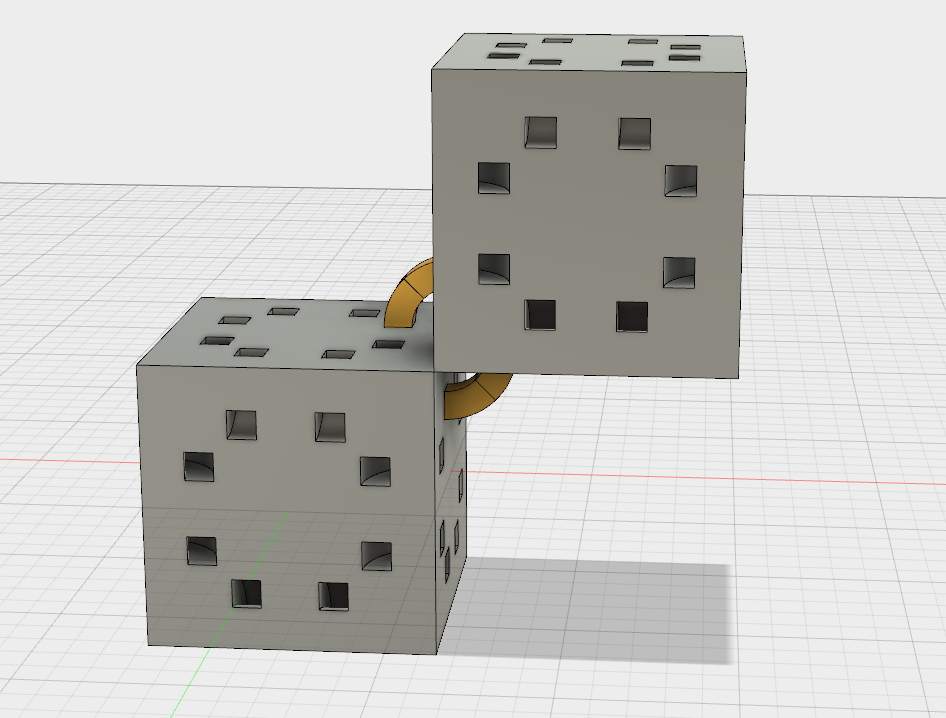
\includegraphics[width=0.85\textwidth]{img/cubes}
    \url{https://a360.co/2KGdj4q}
\end{frame}

\begin{frame}{Druhý koncept}
    \centering
    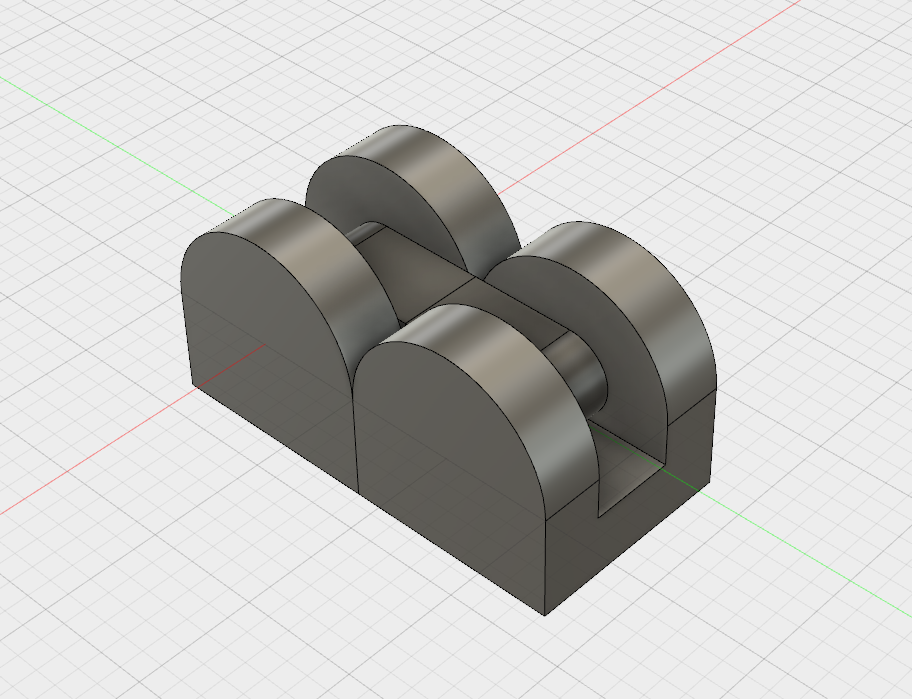
\includegraphics[width=0.85\textwidth]{img/mtranszfi}
    \url{https://a360.co/2k9dRVf}
\end{frame}

\begin{frame}{Zamykací systém -- základ rekonfigurovatelné platformy}
    Požadované vlastnosti:
    \begin{itemize}
        \item mechanická odolnost
        \item symetričnost (rotační \& pohlaví)
        \item odolnost vůči nezarovnání
        \item spotřeba energie
        \item rychlost
    \end{itemize}
\end{frame}

\begin{frame}{Možné zamykací systémy}
    \centering
    \only<1>{
        \begin{block}{Háčky}
            \begin{figure}
                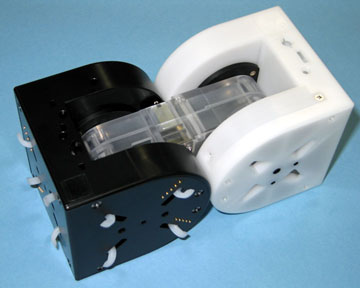
\includegraphics[width=0.7\textwidth]{img/mtran1}
            \end{figure}
        \end{block}
    }
    \only<2>{
        \begin{block}{Permaelektrické magnety}
            \begin{figure}
                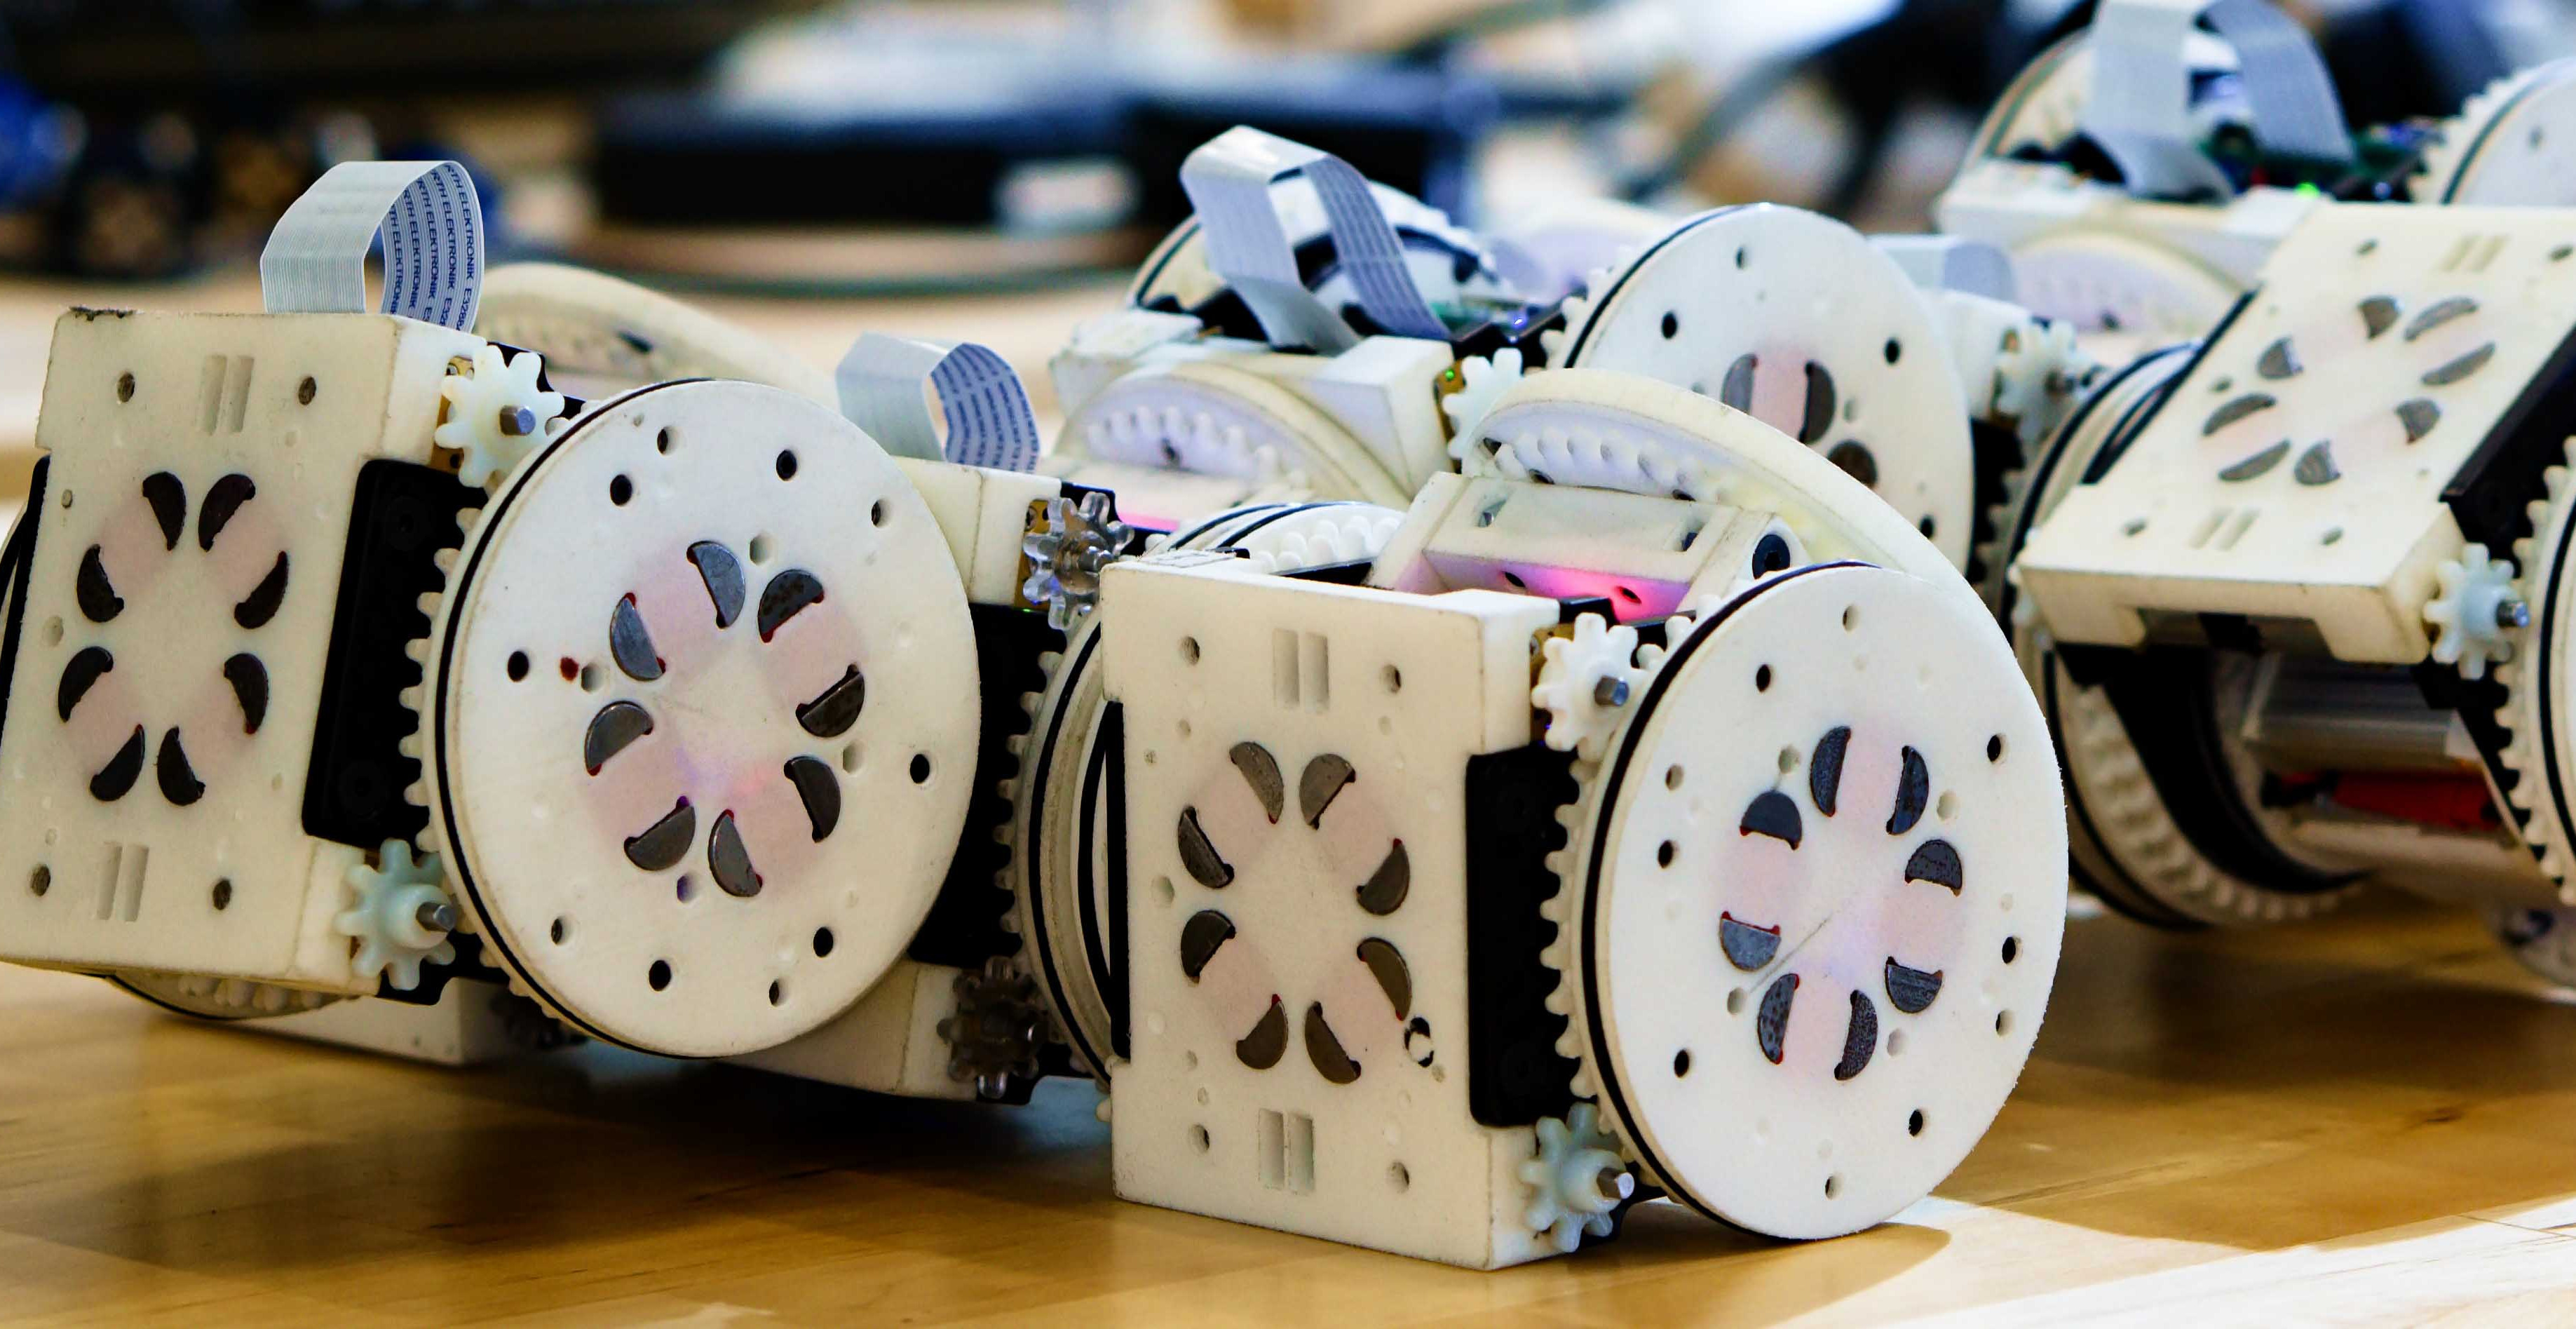
\includegraphics[width=0.85\textwidth]{img/smores1}
            \end{figure}
        \end{block}
    }
\end{frame}

\begin{frame}{Šroubovací systém 1}
    \centering
    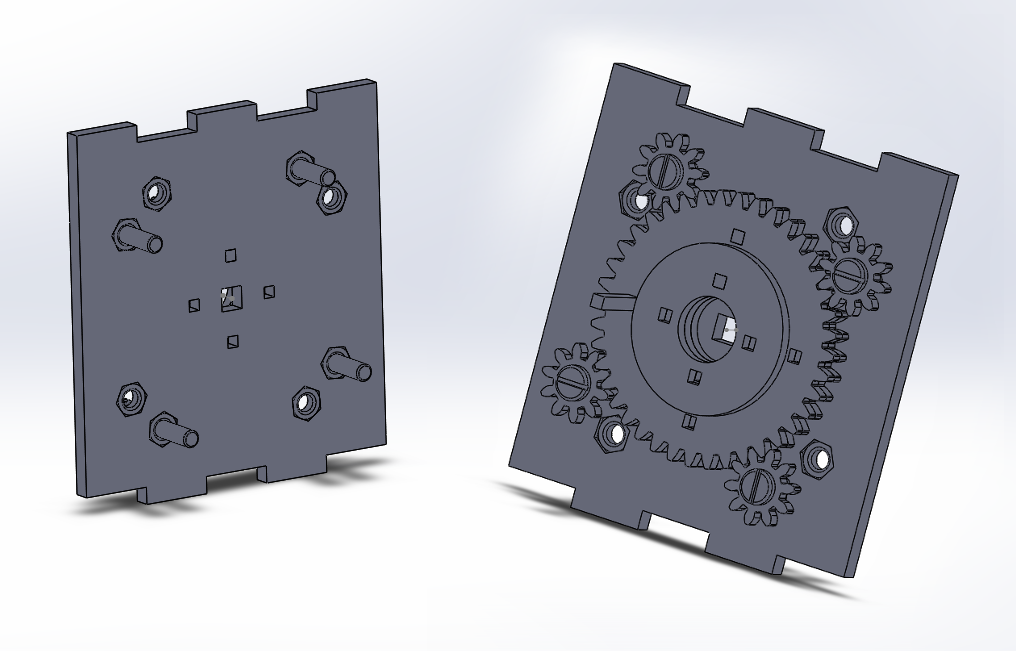
\includegraphics[width=\textwidth]{img/screw1}
\end{frame}

\begin{frame}{Šroubovací systém 2}
    \centering
    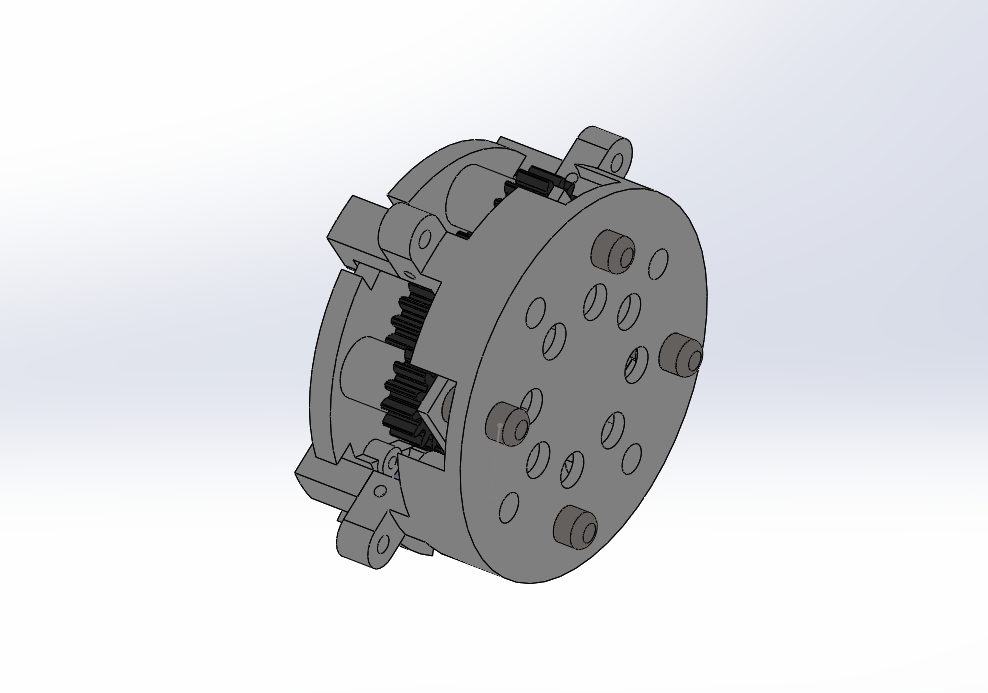
\includegraphics[width=\textwidth]{img/screw2}
\end{frame}

\begin{frame}{Háčkový systém}
    \centering
    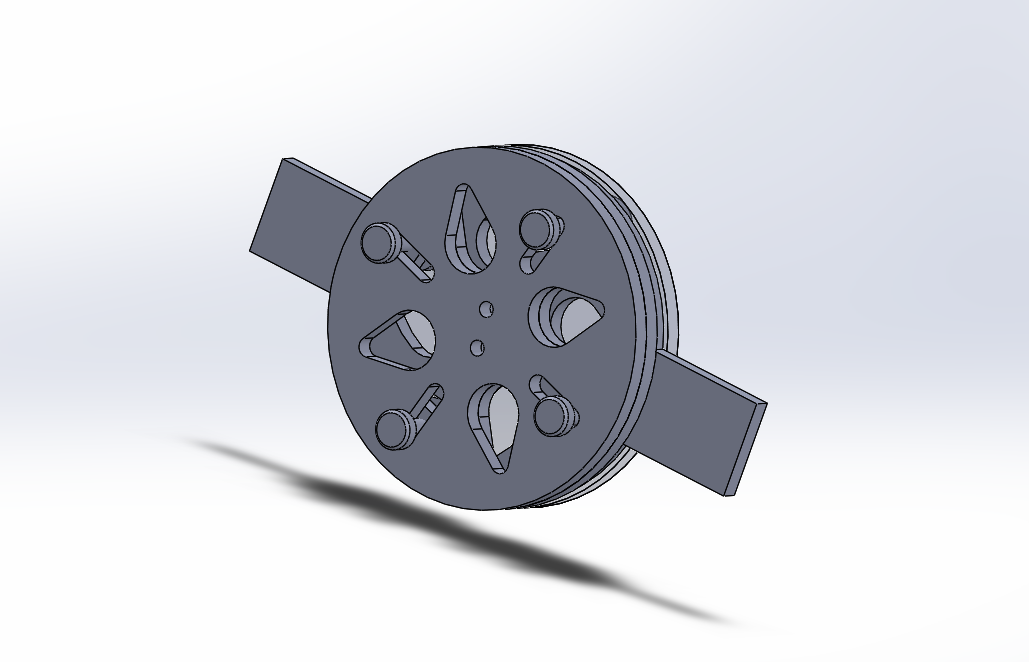
\includegraphics[width=\textwidth]{img/clip1}
\end{frame}

\begin{frame}{Grid-awareness}
    \begin{center}
        \only<1>{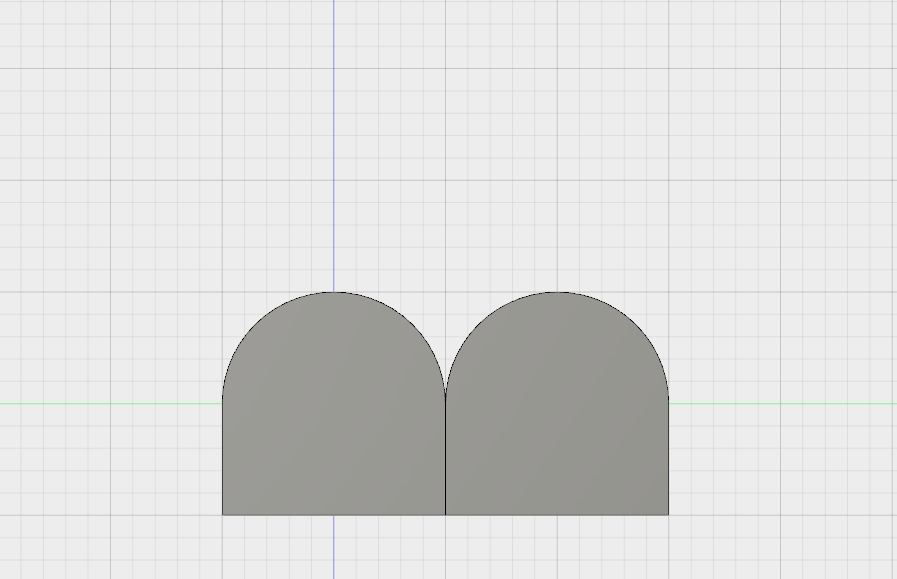
\includegraphics[width=0.8\textwidth]{img/grid_aware_1}}

        \only<2>{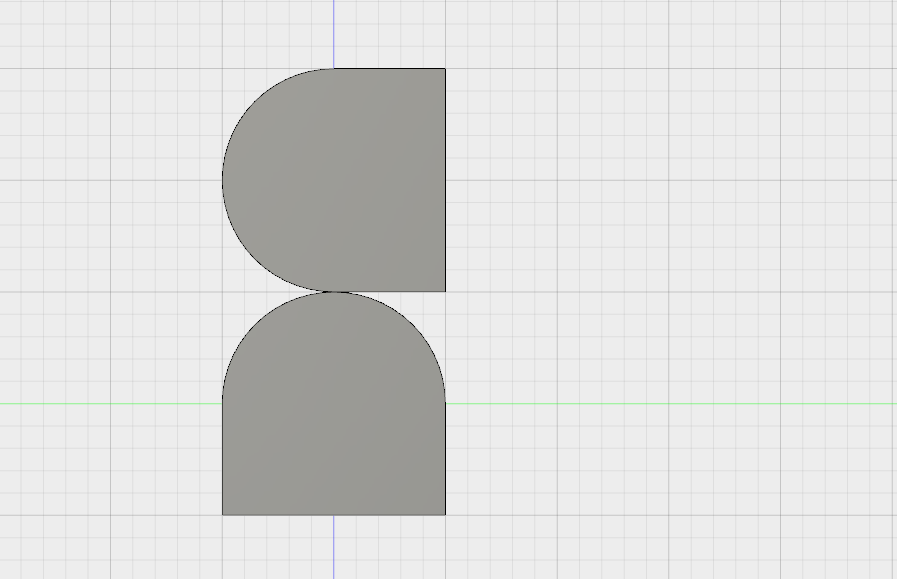
\includegraphics[width=0.8\textwidth]{img/grid_aware_2}}

        \only<3>{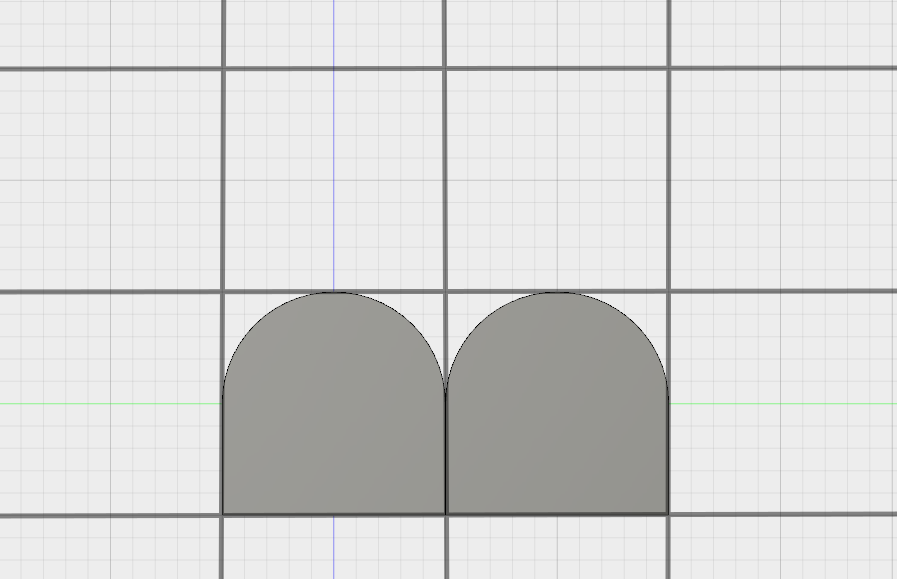
\includegraphics[width=0.8\textwidth]{img/grid_aware_3}}

        \only<4>{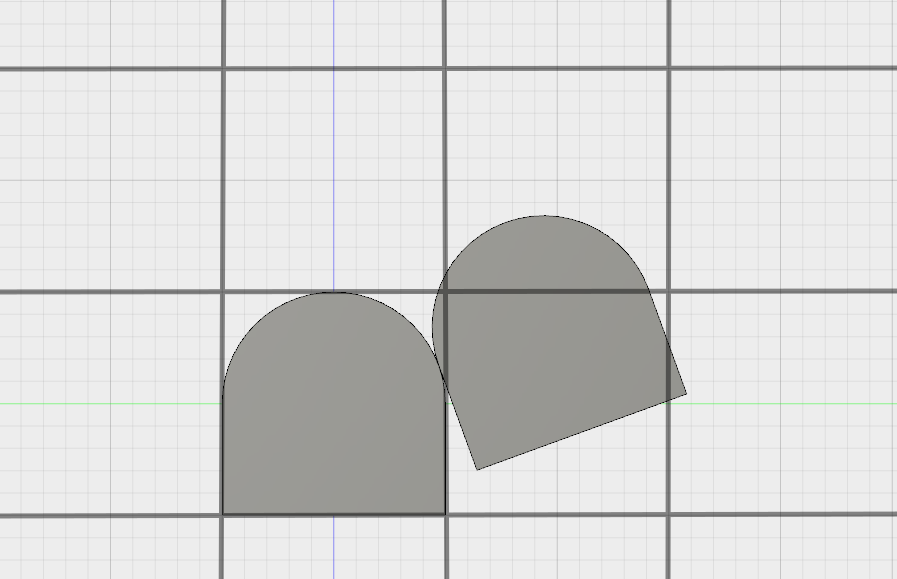
\includegraphics[width=0.8\textwidth]{img/grid_aware_4}}

        \only<5>{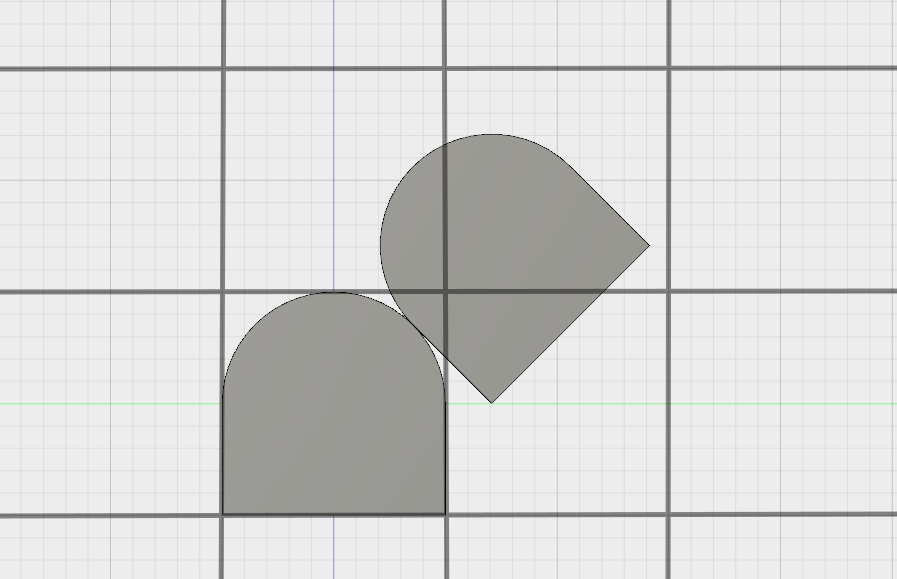
\includegraphics[width=0.8\textwidth]{img/grid_aware_5}}

        \only<6>{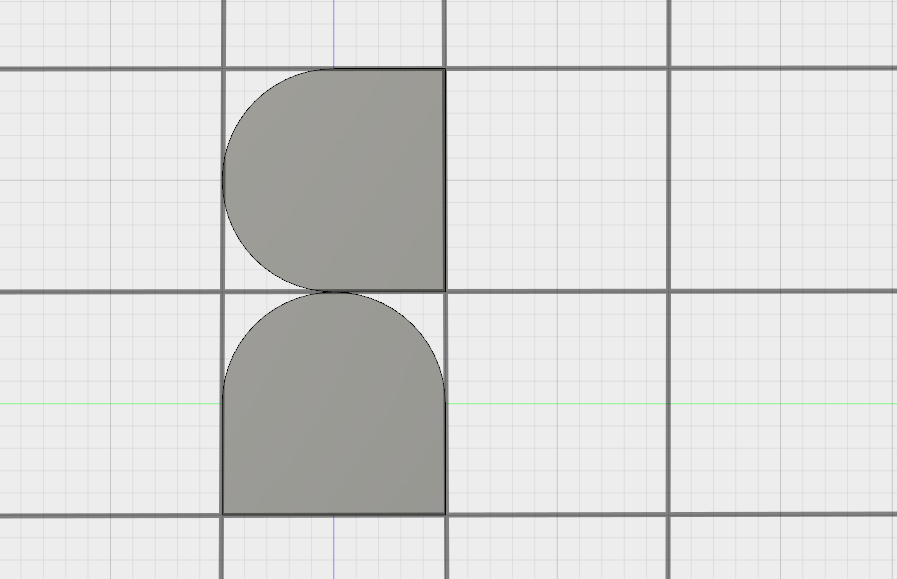
\includegraphics[width=0.8\textwidth]{img/grid_aware_6}}

        \only<7>{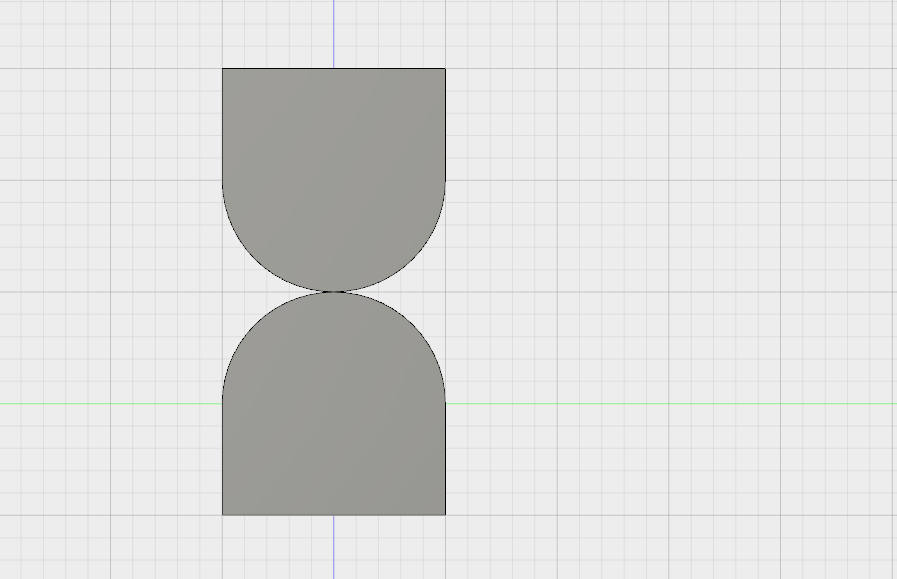
\includegraphics[width=0.8\textwidth]{img/grid_aware_7}}

        \only<8>{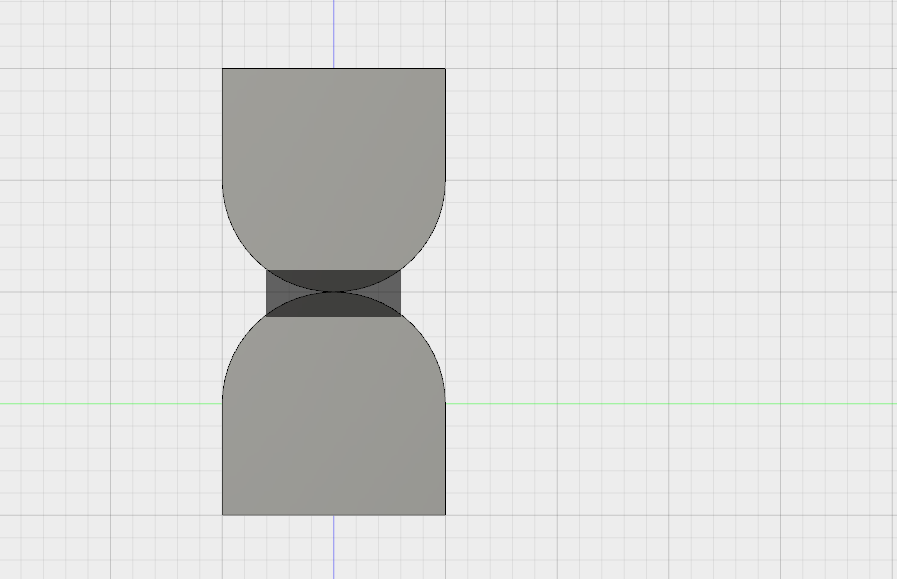
\includegraphics[width=0.8\textwidth]{img/grid_aware_8}}
    \end{center}

    \only<7->{Řešení: robot vepsaný do dvou koulí}

    \only<8->{Problém: je třeba zamykat na dálku}
\end{frame}

\begin{frame}{Háčkový systém 2}
    \centering
    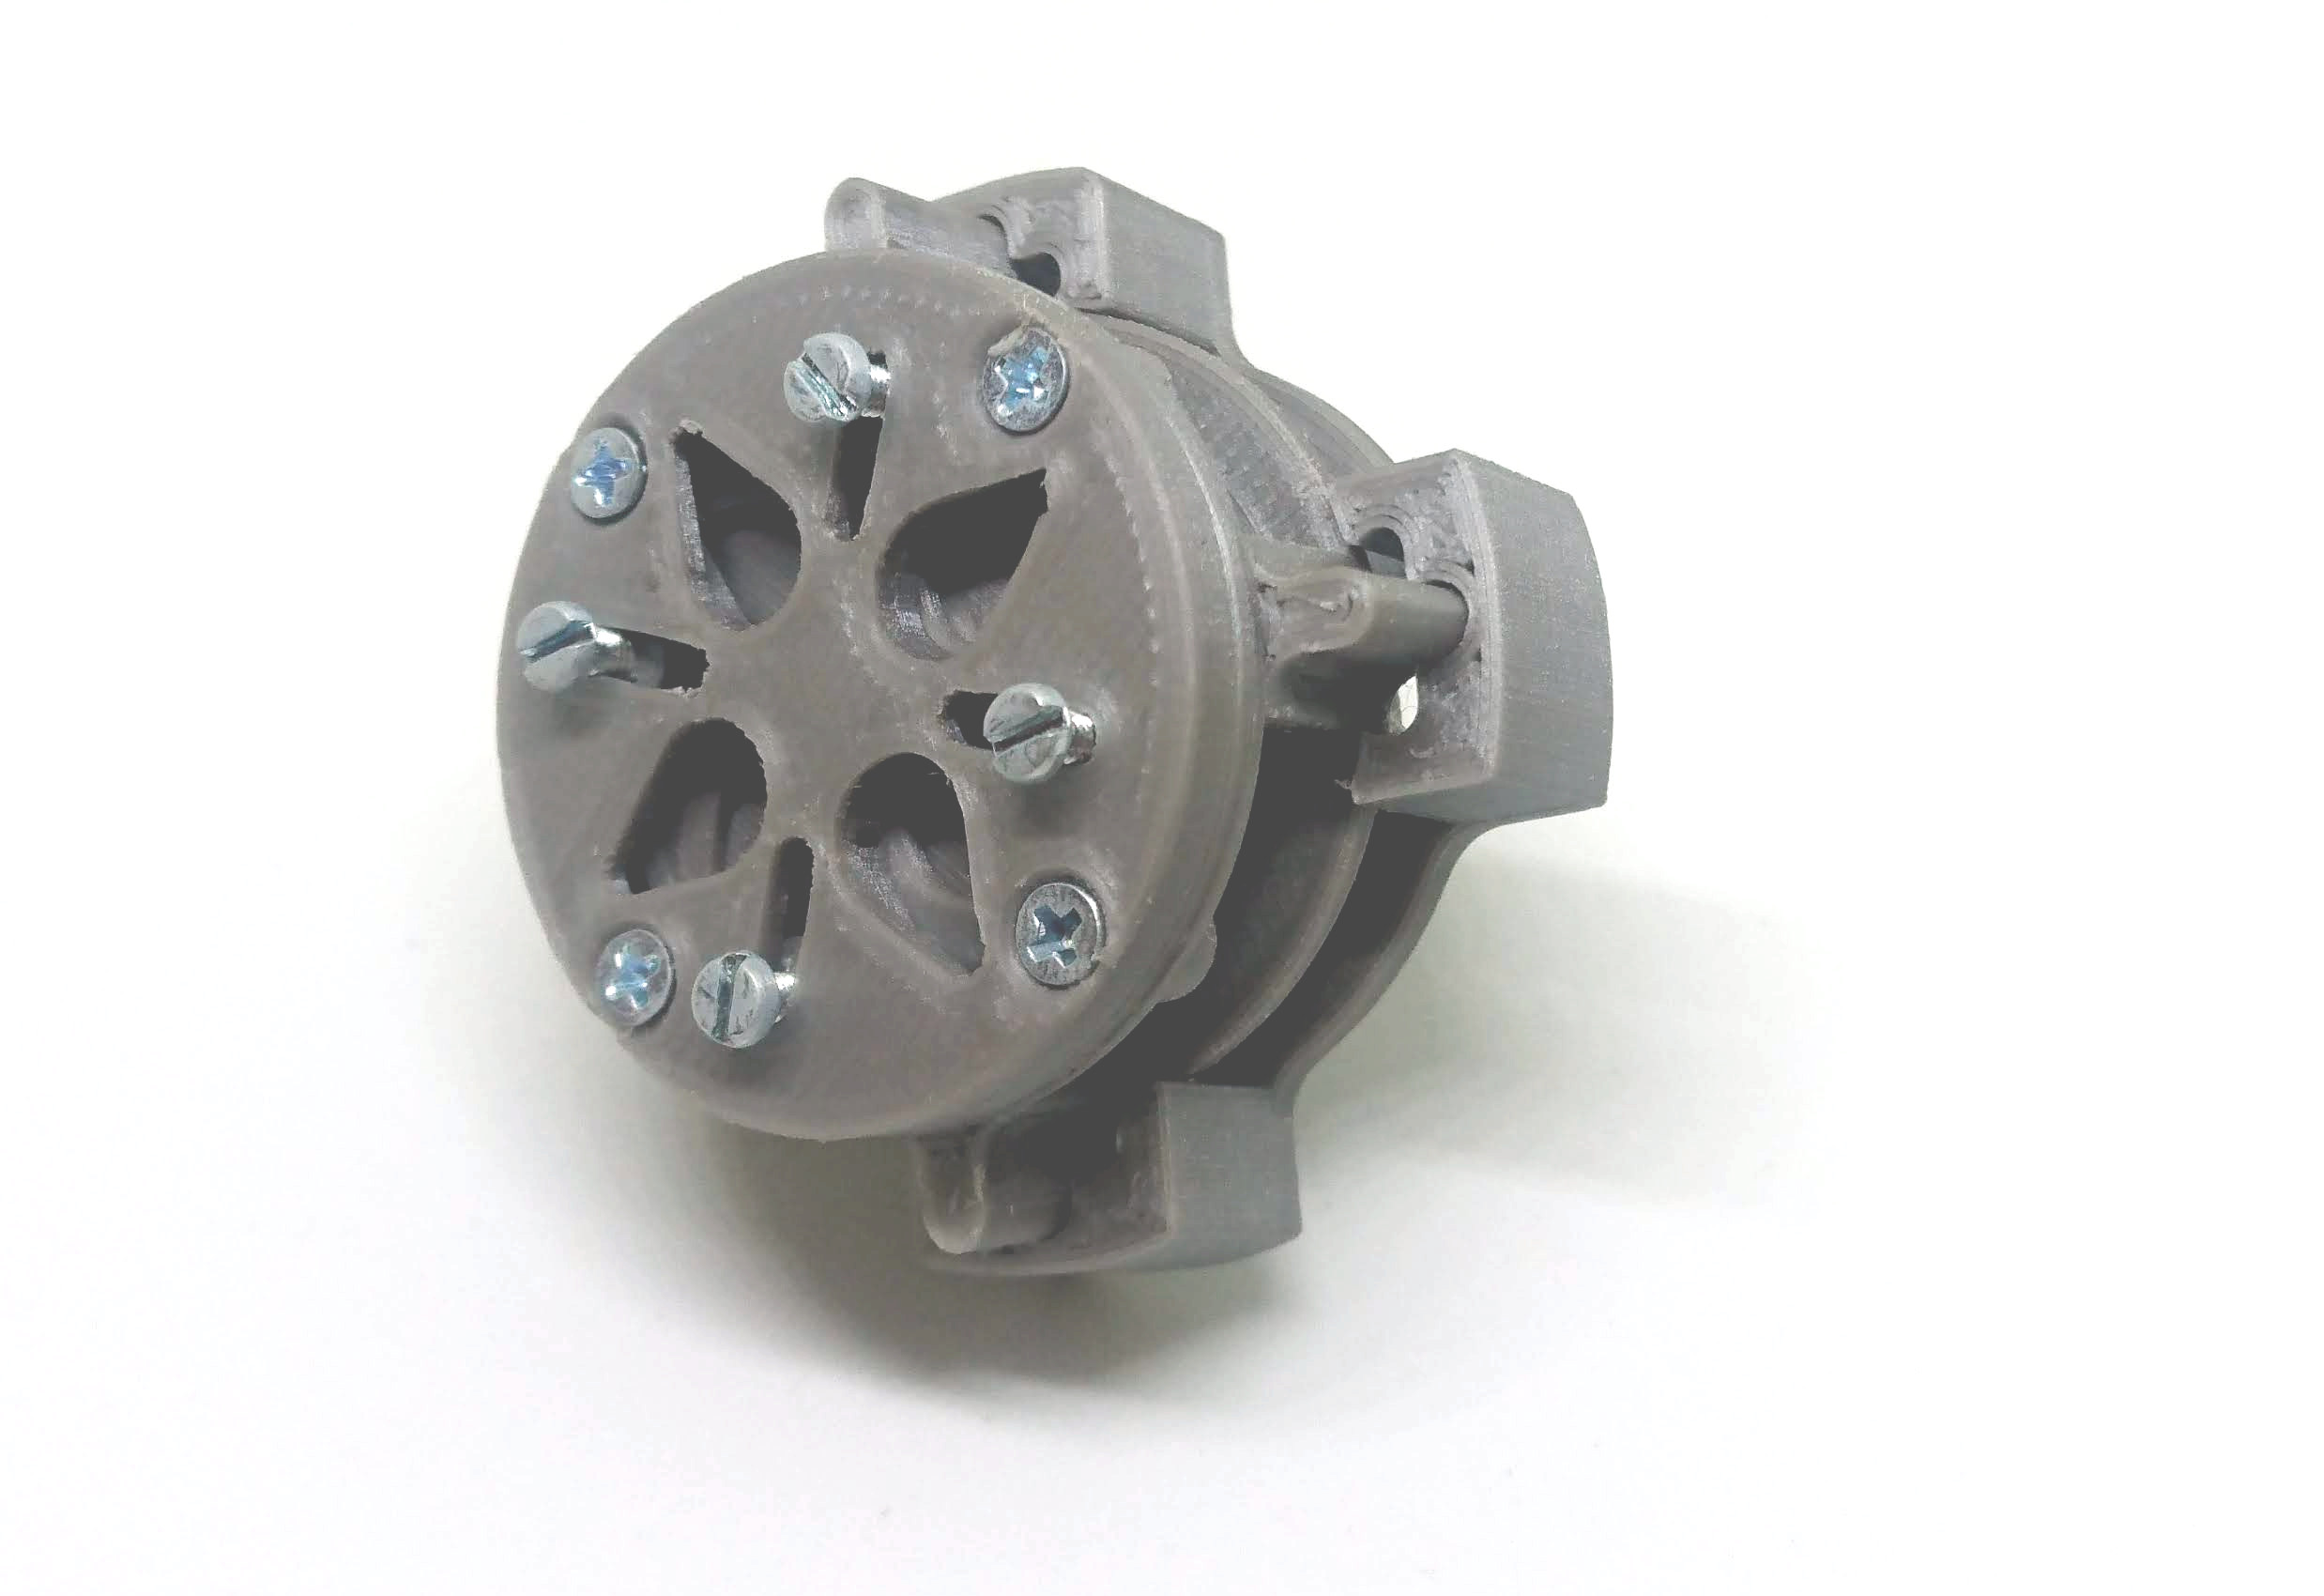
\includegraphics[width=\textwidth]{img/clip2}
\end{frame}

\begin{frame}{Háčkový systém 3}
    \centering
    \only<1>{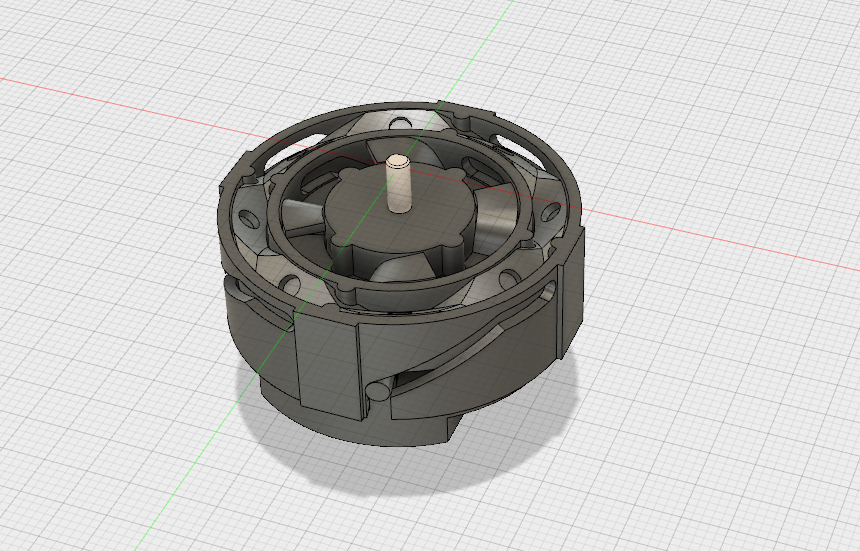
\includegraphics[width=\textwidth]{img/higen1}}
    \only<2>{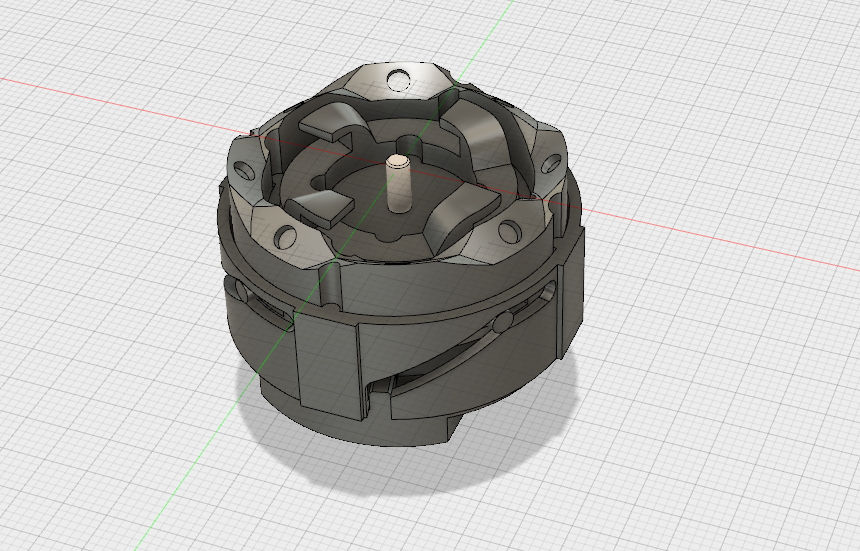
\includegraphics[width=\textwidth]{img/higen2}}
    \only<3>{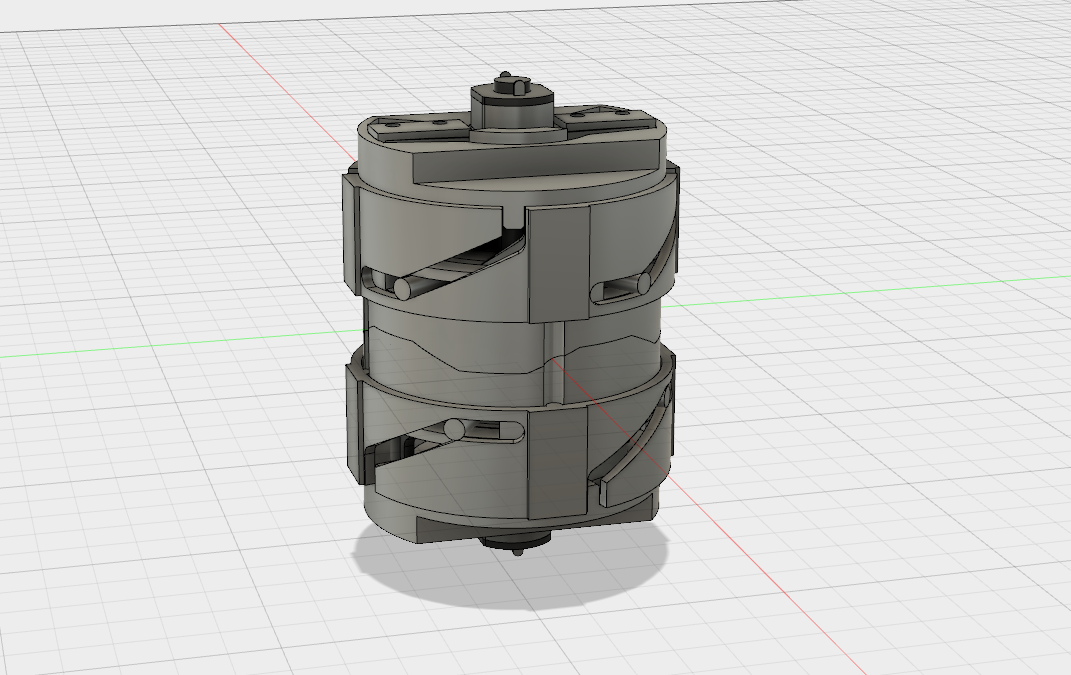
\includegraphics[width=\textwidth]{img/higen3}}
    \url{https://a360.co/2KCw0Gk}
\end{frame}

\begin{frame}{Aktuální stav}
    \begin{figure}
        \centering
        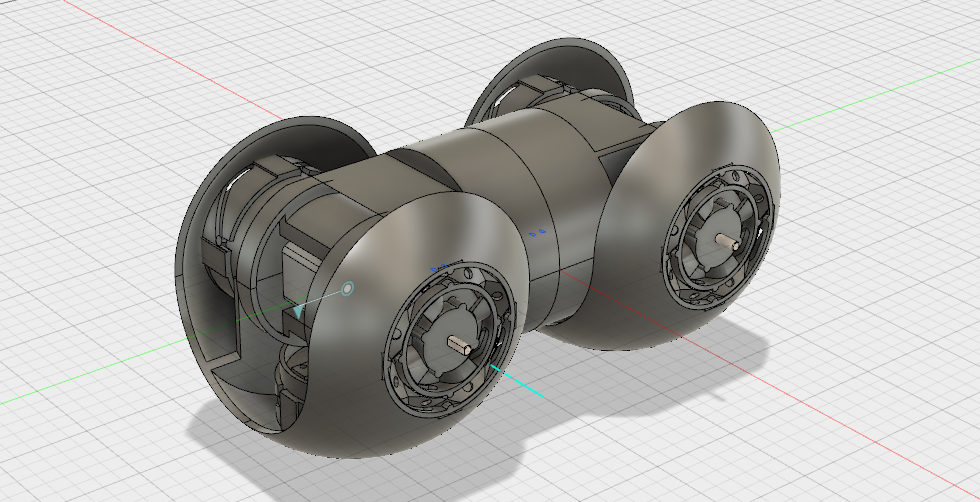
\includegraphics[width=\textwidth]{img/rofi3}
    \end{figure}

    \url{https://a360.co/2KFJ2Th}

    Jsme (snad) pár týdnů od prvních pohybů a vývoj RoFiOS začíná.
\end{frame}

\section{O rekonfigurovatelnosti}

\begin{frame}{ToDo}
\end{frame}

\end{document}

